\section{Technique}%{{{
\label{sec:technique}

Afin que la soirée se déroule sans encombre il nous faut une connexion
internet avec certains ports pour certains protocoles débloqués, et ce
n'est pas une mince affaire. Tout d'abord nous avons demander l'avis de
monsieur Mathieu et la procédure à suivre dans ce genre de cas. Au fil
des échanges nous avons donc fixé le lieu, le périmètre, la date, la
durée, le nombre d'ordinateurs et quelques autres points techniques.
Dans un premier temps, les tests se font dans notre salle de tp
habituelle et notre intermédiaire pour les détails techniques est
monsieur Eric Triquet. Les premiers tests se font sur une seule machine,
un ordinateur portable personnel, on utilise une adresse ip publique et les
tests sont plutôt satisfaisants. Le déploiement vers la maison des
étudiants pose problème. Le responsable sécurité ne veut pas ouvrir
quatres adresses ip public vers des ordinateurs personnels, ce qui veut
dire que nous devons penser à autre chose.  La solution à ce problème a
été trouver en allant directement au CRI avec monsier Triquet afin de
s'expliquer sur les besoins de la soirée.  Nous avons donc établi un
terrain d'entente, la solution est d'utiliser un VLAN, c'est un réseau
indépendant et isolé du reste du réseau et permet de garder un contrôle
sur les données transmises lors de notre soirée.  Les tests en salle tp
se sont montrés concluants, et le déploiement sur la maison des
étudiants n'a pas été long. Les tests finaux sur site se sont montrés
également concluant.
Pour que la soirée se déroule dans les règles de l'art, il nous fallait
du matériel spécifique. En effet, comme expliqué dans la section
barcraft (link) des ordinateurs, une connexion à internet et un
vidéoprojecteur sont requis (et de la bière si possible) pour prétendre
organiser ce type d'évènement.

% section technique (end)%}}}
\section{Matériel}%{{{
\label{sec:materiel}

  Starcraft II est un jeu assez récent comme nous l'avons vu dans la
partie (link) ce qu'il fait qu'il requiert des machines puissantes pour jouer
dans bonnes conditions. Nous avons tout d'abord cherché à emprunter des
machines auprès de l'AEI mais celles-ci - à part pour faire tourner brood
war - sont mauvaises étant donné qu'elles ne contiennent qu'un chipset
graphique (explication). Par la suite nous avons discuté avec les
intervenants pour que ceux-ci ramènent leurs configurations. Cela nous
aurait permis de nous soulager un peu mais aussi d'améliorer la qualité
de jeux du joueur professionnel. Il est connu que l'on joue mieux avec sa
propre machine - avec laquelle on a l'habitude de jouer - plutôt qu'avec la machine d'un
autre.

Les autres matériels dont nous avions besoin comme le vidéoprojecteur,
les micros, la connectique et les tables/chaises étaient disponibles directement à
la Maison des Etudiants ce qui nous a grandement facilité la tâche.

Pour ce qui est de l'isolation des joueurs, nous avons décidé un peu à
la dernière minute qu'un casque de chantier et des écouteurs
intra-oriculaires suffirait. C'est ce qui est utilisé la plupart du
temps sauf pour les gros évènements où on y trouve des "box
insonorisées". Étant donné que notre projet n'est pas de la même
envergure, nous nous en sommes passé bien évidemment.

% section materiel (end)%}}}
\section{Salle et bar}%{{{
\label{sec:salle_et_bar}

Nous cherchions un local possédant le maximum de matériel dont nous
avions besoin pour la soirée pour plus de facilité. Nous avons tout
dabord cherché a au sein du campus de Lille 1 avant de se diriger vers
un commerce qui nous aurait demandé beaucoup plus d'efforts d'un point de
vue recherche (le concept étant peu connu du grand public cela aurait été
très difficile).

Ayant participé a certaines soirées étudiantes qui se déroulent le jeudi
soir à la Maison des Etudiants (MDE), nous avons remarqué que celle-ci
était disponible assez facilement, gratuitement et avec du matériel
approprié. En effet, les thématiques proposées par la MDE sont très
diverses. Elle peut aussi bien faire office de salle de réunion que de
concert ou même de soirée cinéma.

Cependant, pour avoir le droit d'organiser un évènement dans celle-ci, il est nécessaire 
d'appartenir à une association étudiante du campus suffisamment sérieuse. Aucun
membre du groupe n'étant membre d'une quelconque association nous étions un
peu inquiets. Après s'être renseigné à différents endroits, il faut
simplement se rapprocher d'une association pour qu'elle puisse se porter
garante de l'évènement.

La nécessité d'avoir une association soutenant notre projet fut obligatoire pour
l'obtention d'une extension d'assurance pour les biens et les personnes
au cas où un problème majeur surviendrait lors de la soirée.

L'AMUL est l'association qui prend en charge le bar de la Maison des
Etudiants. Pour pouvoir assurer une permanence pour notre soirée, nous
avons du contacter le président de cette association afin de demander
son accord. Un échange par mail est alors effectué afin de conclure avec
un rendez-vous pour définir nos attentes concrètes ainsi que leur faisabilité. 
Suite à cet entretien il a été convenu qu'une permanence
aurait lieu de 18h à 22h.

% section salle_et_bar (end)%}}}
\section{Partenariats et sponsors}%{{{
\label{sec:partenariats_et_sponsors}

- Demande de financement du projet auprès de la FSDIE (Fonds de solidarité
et de Développement des Initiatives Etudiantes)

Nous nous sommes tout dabord rendus au bâtiment A3 pour récupérer un
dossier de demande de financement destinés à la réalisation des projets d'étudiants. 
Ce dossier requérait un certain nombre de pièces justificatives comme le
planning de déroulement de la soirée, le montant envisagé, le potentiel
nombre de participants. Une fois le dossier rempli, nous devions encore passer devant 
une commission qui validerait ou non le financement de notre projet. Nous avons donc
abandonné cette possibilité car nous ne savions pas si le projet était
possible. En effet, trop de paramètres étaient encore flous, tels que les commentateurs
ou la certitude d'avoir une connexion à Internet publique. Cela n'aurait donc pas été
sérieux de leur faire perdre du temps avec un dossier incomplet.

- collaboration avec l'aei

Nous avons choisis de collaborer avec l'AEI (Association des Etudiants
en Informatique), habituée à ce genre de soirée à thématique *geek* et 
emprunteur historique de la Maison des Etudiants.
Leur principal local se situe dans le bâtiment M5, au centre de la
cité scientifique ou sont concentrés la pluspart des informaticiens de
Lille 1.
Nous avons donc exposé notre projet avec ceux-ci

- demande de financement auprès de Micromania (v2)

Une demande de financement à été faite auprès du célèbre magasin de
jeux-vidéo Micromania qui nous a vallu un refus. Cette
enseigne ne sponsorisant pas d'évènements de genre.

%TODO
- demande de sponsor Materiel.net (Lomme)

Nous avons également contacté Materiel.net afin de savoir s'ils pouvaient nous prêter,
louer du matériel ou encore sponsoriser la soirée mais ils n'étaient pas intéressés.

%TODO
- envoie d'un mail au service communication sans reponse

N'ayant trouvé aucun moyen de financement pour permettre aux
intervenants et nous-mêmes de nous restaurer lors de la soirée, nous
n'avions pas d'autre choix que de répartir les coûts entre membre du
projet. C'est à ce moment la que le responsable de la formation DA2I
proposa de débloqué les fonds allouées à la licence pour permettre de
financer les évènements des étudiants. Ce fut une aubaine pour nous.

Nous avons tout dabord pensé à acheter nous-mêmes les aliments pour
ensuite ce faire rembourser avec cette somme mais cela posait des
problèmes logistiques. Une autre idée à donc été proposé : commander des
plateaux repas (qui est un service proposé par l'iut). Il nous a donc
été demandé de réunir des informations auprès des intervenants de la
soirée, comme leur nom, prénom, adresse, fonction pour que cette demande
aboutisse.

% section partenariats_et_sponsors (end)%}}}
\section{Intervenants}%{{{
\label{sec:intervenants}

\subsection{Le rôle des intervenants}%{{{
\label{sub:le_role_des_intervenants}

Nous souhaitions inviter des personnes extérieures pour le projet à
différentes fins. Il nous fallait un ou des commentateurs ainsi que des
joueurs, qui sachant que leurs parties allait être commentées devait faire
le show pour le public. Ceux-ci, pour engrangé du monde, devait être
connu de la scène française.

% subsection le_role_des_intervenants (end)%}}}
\subsection{Alexandre "Makoz" Schilling}%{{{
\label{sub:alexandre_makoz_chilling}

Un des membres du groupe qui connaissant bien la scène française autour
de Starcraft II, s'est occupé de contacter des intervenants. Celui-ci,
appréciant Alexandre "Makoz" Schilling l'a contacté en premier. Makoz qui
était au moment de la demande manager de *Sparte Legion*, une équipe
française faisant de plus en plus parler d'elle. En plus de ses qualités
managériales il est commentateur professionnel de matchs via des
streams (explication) et propose de decortiquer des matchs entre joueurs
amateurs ou experimentés sur sa page Youtube. Malheureusement, Alexandre
par ses responsabilités n'a pas pu se joindre à nous. Il nous a
cependant invité a contacter certaines de ses connaissances.

% subsection alexandre_makoz_chilling (end)%}}}
\subsection{Le clan All Against Authority}%{{{
\label{sub:le_clan_all_against_authority}

Une deuxième demande a été faite auprès du clan *aAa* qui comporte
plusieurs équipes professionnelles dont une sur Starcraft II et une sur
League of Legends. Les négociations se sont déroulées par échanges de mails. 
Ceux-ci par l'intermédiaire de leur manager ayant pour
pseudo *zidwait* fut interessé. Ils nous ont proposé quatre personnes,
deux commentateurs et deux joueurs situés de toute part en France.
Cependant, l'évènement n'étant pas considéré comme un tournoi mais comme
une prestation de service par leur sponsors, ceux-ci n'ont pas désiré
prendre en charge les frais de déplacement. La somme requise pour faire
venir les personnes consernées était éstimée à hauteur de 500 euros, ce
dépassa de loin notre budget prévisionnel. Nous avons donc été
contraints de refuser cette offre. Il nous ont néanmoins proposé de
retransmettre la soirée sur leur stream si nous filmions l'évènement.
Nous avons refusé pour deux raisons. La première étant la monopolisation de l'un 
d'entre nous toute la soirée, et deuxièmement, personne dans le groupe n'a pour
vocation de devenir caméraman.

% subsection le_clan_all_against_authority (end)%}}}
\subsection{Thomas "Soey" Brandt \& Julien Roy}%{{{
\label{sub:tthomas_soey_brandt_&_julien_roy}

Lorsque nous avons exposé à Makoz nos problèmes pour trouver des intervenants, 
celui-ci nous a conseillé de contacter Thomas "Soey" Brandt qui
est un joueur semi-professionnel sur Lille. Thomas a été séduit par
notre offre qu'il a accepté assez vite lorsque nous lui avons présenté
le projet. Par contre Thomas et son collègue n'habitaient pas vraiment à
Lille mais à Dunkerque. Il fallait donc quelqu'un pour aller les
chercher le jour de l'évènement, puis les reconduire une fois la soirée
terminée. Un des membres du groupe ayant sa famille sur Dunkerque, il a
accepté de faire la navette. Thomas a accepté sans rien demander en
échange à part qu'il puisse jouer à Heart of the Swarm "intensivement".
En effet, le jeu étant sorti la veille de la soirée "Soey" avait besoin
de s'entrainer dur pour ne pas prendre du retard sur les autres joueurs.

% subsection ttthomas_soey_brandt_&_julien_roy (end)%}}}

% section intervenants (end)%}}}
\section{Communication}%{{{
\label{sec:communication}

\subsection{L'affiche}%{{{
\label{sub:l_affiche}

La communication étant importante pour la réalisation du projet, nous sommes partis sur l'élaboration
d'une affiche A3.

Nous avons souhaité que cette affiche se devait d’être contrastée et peu chargée afin qu’elle soit
claire et lisible de loin, c’est pourquoi la combinaison du noir sur fond blanc fut adaptée à ce choix.
De plus, il fallait que l’identité visuelle de l’affiche puisse parler aux joueurs, d’où l’utilisation
d’une police spéciale de grande taille, police de la licence \og Starcraft \fg{}, et placée en haut de l’affiche.

La date et le lieu bénéficient également d’une taille plus grande que le texte du corps de l’affiche.
Concernant ce dernier, nous avons décidé de ne pas le charger en texte afin de bénéficier d’une police
plus grande grâce à l’espace obtenu.
Nous avons mis en avant la venue du commentateur et joueur Soey  de niveau \og top master \fg{}  dans le but
de donner une plus grande crédibilité à l’évènement.
Enfin, pour rajouter à l’identité visuelle, nous avons fait figurer les emblèmes des trois races du jeu,
ainsi qu’une grande bannière où apparaît le protagoniste principal de la prochaine extension.
21 affiches ont été imprimées au format A3, pour ensuite être affichées dès le 1er mars à l’IUT A, au M1,
au M3, au M5, à la MDE et dans quelques résidences universitaires.

% subsection l_affiche (end)%}}}
\subsection{L'enquête d'audience}%{{{
\label{sub:l_enquete_d_audience}

L'affiche seule n'étant pas suffisante pour la communication, nous nous sommes tournés vers la
Maison Des Étudiants et son e-mai afin de diffuser l'information à tous les étudiants de l'université.
Profitant de ce moyen, nous avons élaboré un questionnaire. Le but de celui-ci était d'obtenir une estimation
du nombre de participants et trouver un potentiel commentateur.

Malheureusement, le mail n'a été envoyé que le 5 mars, soit une semaine avant l'évènement.
Nous avions néanmoins déjà trouvé notre commentateur.

L'enquête est un questionnaire comporte quatre à neuf questions selon les réponses des sondés. 30 ont répondu.
Voici les réponses à quelques questions :

Êtes-vous intéressé par une soirée Starcraft 2 (WoL, HotS) ?

\begin{figure}
  \begin{center}
    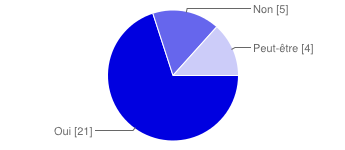
\includegraphics[scale=1.57]{images/chart_1.png}
    \caption{}
    \label{flow}
  \end{center}
\end{figure}

La soirée se déroulera un mercredi soir (18h-23h), serez-vous présent ?

\begin{figure}
  \begin{center}
    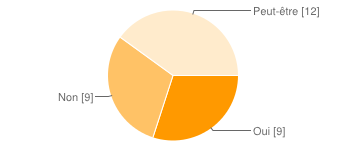
\includegraphics[scale=1.57]{images/chart_2.png}
    \caption{}
    \label{flow}
  \end{center}
\end{figure}

Aimeriez-vous y jouer au cours de cette soirée ?

\begin{figure}
  \begin{center}
    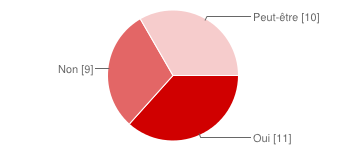
\includegraphics[scale=1.57]{images/chart_3.png}
    \caption{}
    \label{flow}
  \end{center}
\end{figure}

Nous pouvons tirer de ces informations une estimation de plus ou moins 15 personnes présentes si l’on prend
la moitié des \og peut-être \fg{} + les \og oui \fg{}.
En sachant que tous les étudiants ne prêtent pas attention aux mailings de l’université, on peut ajouter
une quinzaine de personnes pour atteindre une estimation de 30 participants.
% subsection l_enquete_d_audience (end)%}}}
\subsection{Les contraintes/ratés}%{{{
\label{sub:les_contraintes_rates}

Un autre moyen de communication fut utilisé, la création d'un évènement
Facebook. Néanmoins cela n'a pas fonctionné, la propagation de cet
évènement ne fut pas suffisante sur le réseau social. De plus cette page
de promotion a été ouverte très tardivement ce qui fait que  nous
n'avons pas eu le temps de faire marcher les connaissances.

La contrainte majeur concernant l'élaboration de la communication fut l'attente
de la confirmation de tous les éléments du projet.  Nous ne pouvions
notamment pas lancer la production des affiches sans savoir si nous
avions un commentateur par exemple.

% subsection les_contraintes_rates (end)%}}}

% section communication (end)%}}}
\section{Bilan financier}%{{{
\label{sec:bilan_financier}

%TODO
Bilan financier
        Prévisionnel
            - salle
            - bar
            - matos
            - intervenant
            - comm
            - repas
        Reel
           ...

% section bilan_financier (end)%}}}
\section{Bilan de la soirée}%{{{
\label{sec:Bilan_de_la_soiree}

\subsection{Prévisionnel}%{{{
\label{sub:previsionnel}

La date de la soirée devait être judicieusement choisie afin d'obtenir une affluence satisfaisante.

Ayant vu grâce au mailing de l’université que la MDE accueillait des soirées chaque jeudi
nommées \og Jeudifférents \fg{}, nous nous sommes dit qu’une soirée comme la notre collait
parfaitement à cette appellation. Malheureusement, nous avions commencé à prendre contact
début février pour la réservation, ce qui fut trop tard. Tous les jeudis sur deux mois étaient
déjà réservés.
Il nous a donc fallu choisir un autre jour de la semaine. Après renseignements auprès de la
MDE, seuls le mercredi et le vendredi étaient libres la semaine du 11 au 17 mars. Le choix ne
fut pas difficile, le mercredi fut choisi naturellement car les étudiants ayant un appartement
dans la métropole rentrent chez eux le vendredi. De plus, le mercredi 13 mars correspondait
au lendemain de la sortie de la nouvelle extension du jeu.
A propos de l’horaire de la soirée, nous avions décidé de commencer dès 18h pour finir à
22h. En effet, le fait de commencer à 18h permet aux étudiants de se rendre à la soirée juste
après les cours. Ensuite, d’après l’AEI, la MDE ferme à 23h et pour ouvrir au-delà de cette
heure, il était nécessaire d’avoir une dérogation pénible à obtenir. Nous nous sommes donc
donné une heure afin d’avoir le temps de remballer, mais également de partir plus tôt pour
reconduire les intervenants chez eux, à Dunkerque.
Après s’être mis d’accord sur la date et l’heure de la soirée, nous devions discuter du
programme.
Il ne fut pas aisé de définir un programme à heures fixes, car les parties n’ont pas une durée
définie. Elles peuvent durer entre 5 et 50 minutes, la moyenne se situant à 25 minutes de jeu.
C’est pourquoi nous avons décidé d’énoncer le contenu de la soirée sans y faire figurer
d’heure.
Nous avions donc prévu de commencer par 20 minutes d’introduction en vidéo sur le jeu et
ses mécanismes afin de pouvoir rendre la soirée plus compréhensible pour les néophytes.
Puis enchainer avec les matchs commentés des intervenants pour finir avec des matchs
confrontant des joueurs du public. Nous avons choisis cet ordre car nous pensions que le plus
amusant était de faire jouer le public, et que cela permettrait de les retenir un maximum.

% subsection previsionnel (end)%}}}
\subsection{Réel}%{{{
\label{sub:reel}

Arrivé le jour J, nous avons été confrontés à plusieurs imprévus.
La météo ne fut pas clémente le 12 mars ainsi que le 13 mars, la neige étant fortement
tombée ces jours là. La circulation était devenue difficile dans la région et beaucoup de cours
furent perturbés.
Ceci impacta fortement l’affluence de la soirée, et surtout son déroulement. Les intervenants
ne purent pas venir du fait des conditions climatiques. Le retour à la fin de la soirée aurait été
dangereux à cause du verglas, et aucun hébergement n’eut pu être possible.
Ces imprévus nous ont donc forcés à improviser.

Les préparatifs commencèrent à 16h, tout se passa bien ou presque. Une fois nos PC personnels
installés, nous nous aperçûmes qu’il fallût utiliser une connectique autre que VGA afin de
connecter nos PC au vidéoprojecteur de la MDE. Heureusement, le directeur de la MDE M.Bross
possédait un vidéoprojecteur VGA avec une bonne qualité de projection.
Une dizaine de personnes arrivèrent passé 18h. Comme prévu à cause du climat, peu de
personnes assistèrent à la soirée. Nous avons recensé une vingtaine de personnes
différentes, mais jamais plus de 11 personnes simultanément.
A cause des imprévus et compte tenu de la faible affluence, nous avons décidé de faire jouer
directement les personnes présentes en projetant leurs parties sur vidéoprojecteur comme
prévu. Julien étant parmi nous le plus expérimenté, il put donc commenter quelques matchs
au cours de la soirée.
Vers 18h50, nous fûmes encore victime d’un imprévu. Les serveurs de jeu de tous les jeux en
ligne de Blizzard tombèrent, nous empêchant de jouer pendant 30 minutes. Pendant ce
temps, nous diffusions les vidéos explicatives de Starcraft II, ce qui permit de combler le
blanc engendré. Néanmoins, un groupe de 4 personnes s’en alla durant ce laps de temps.
Une fois la situation rentrée dans l’ordre, nous pûmes continuer la soirée en petit comité et
terminer à 23h. Entre temps, nous fûmes une pause restauration vers 21h30. Nous
partageâmes les deux plateaux repas en trop avec les participants du fait de l’absence des
deux intervenants. La soirée termina à 23h car nous apprîmes en arrivant pour les préparatifs
que nous pouvions utiliser la salle jusqu’à minuit.
% subsection reel (end)%}}}

% section Bilan_de_la_soiree (end)%}}}
